\documentclass{article}
\usepackage[UTF8]{ctex}
\usepackage{geometry}
\usepackage{natbib}
\usepackage{float}
\geometry{left=3.18cm,right=3.18cm,top=2.54cm,bottom=2.54cm}
\usepackage{graphicx}
\pagestyle{plain}	
\usepackage{setspace}
\usepackage{amsmath}
\usepackage{caption2}
\usepackage{tikz}
\usetikzlibrary{shapes.geometric, arrows}
\usepackage{datetime} %日期
\renewcommand{\today}{\number\year 年 \number\month 月 \number\day 日}
\renewcommand{\captionlabelfont}{\small}
\renewcommand{\captionfont}{\small}
\begin{document}
\tikzstyle{startstop} = [rectangle,rounded corners, minimum width=3cm,minimum height=1cm,text centered, draw=black,fill=white!30]
\tikzstyle{process} = [rectangle,minimum width=3cm,minimum height=1cm,text centered,text width =3cm,draw=black,fill=white!30]
\tikzstyle{arrow} = [thick,->,>=stealth]
\begin{figure}
    \centering
    
\includegraphics[width=8cm]{upc.png}

    \label{figupc}
\end{figure}

	\begin{center}
		\quad \\
		\quad \\
		\heiti \fontsize{45}{17} \quad \quad \quad 
		\vskip 1.5cm
		\heiti \zihao{2} 《计算科学导论》课程总结报告
	\end{center}
	\vskip 2.0cm
		
	\begin{quotation}
% 	\begin{center}
		\doublespacing
		
        \zihao{4}\par\setlength\parindent{7em}
		\quad 

		学生姓名:\underline{\qquad  杨汶昊 \qquad \qquad}

		学\hspace{0.61cm} 号:\underline{\qquad 1907010308\qquad}
		
		专业班级:\underline{\qquad 计算1903 \qquad  }
		
        学\hspace{0.61cm} 院:\underline{计算机科学与技术学院}
% 	\end{center}
		\vskip 2cm
		\centering
		\begin{table}[h]
            \centering 
            \zihao{4}
            \begin{tabular}{|c|c|c|c|c|c|c|}
            % 这里的rl 与表格对应可以看到,姓名是r,右对齐的;学号是l,左对齐的;若想居中,使用c关键字。
                \hline
                课程认识 & 问题思 考 & 格式规范  & IT工具  & Latex附加  & 总分 & 评阅教师 \\
                30\% & 30\% & 20\% & 20\% & 10\% &  &  \\
                \hline
                 & & & & & &\\
                & & & & & &\\
                \hline
            \end{tabular}
        \end{table}
		\vskip 2cm
		\today
	\end{quotation}

\thispagestyle{empty}
\newpage
\setcounter{page}{1}
% 在这之前是封面,在这之后是正文
\section{引言}
经历了8周的《计算机科学导论》的学习,这门课程使我受益良多。在知识上开阔了我的见闻,在思维上深化了我的思辨能力,在沟通上强化了我与他人的沟通表达能力。不仅提高了我的科学素养,而且提高了我的人文素质。在课程即将结束之际,写下结业报告,一对我的学习心得体会,二对老师的课程做总结报告。

\section{对计算科学导论这门课程的认识、体会}
《计算机科学导论》这门课程作为一门导论课程,本身可以认为对计算机这门学科的概况和认识,力求拓宽我们的知识广度,启发和增进学生对各个领域的认识,进而为未来的学习就业奠定坚实的基础。\par
课程总体可以分为四个部分,分别为:科学哲学的思想方法、计算机学科基本概念和发展历程以及当前学科前沿课题的分享。其中最令我印象深刻和深有体会的要数目前学科前沿课题的分享。\par

% \subsection{前沿课题一览}
% 图片插入的样例:\par
% \begin{figure}[h!]
% \centering
% 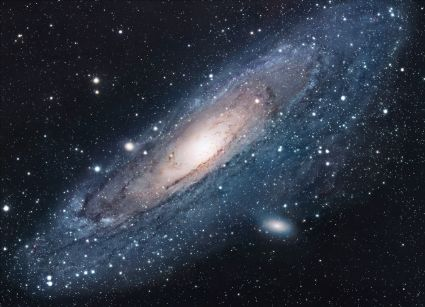
\includegraphics[scale=1.7]{universe}
% \caption{The Universe}
% \label{fig:universe}
% \end{figure}

\subsection{前沿课题一览}
% 表格插入样例:\par

\begin{table}[h]
	% \large
    \centering
    \captionfont
    \caption{前沿课题简表}
\begin{tabular}{|c|c|}
% 这里的rl 与表格对应可以看到,姓名是r,右对齐的;学号是l,左对齐的;若想居中,使用c关键字。
    \hline
    课题名称 & 类别\\
    \hline
    智慧遥感 & 人工智能 \\\hline
    智慧社区 & 人工智能\\	\hline
    智慧银行 & 人工智能\\	\hline
    自动驾驶 & 人工智能\\	\hline
    比特币	& 区块链\\	\hline
    区块链	& 区块链\\	\hline
    数字版权 & 区块链\\	\hline
    Jave学习路线 & 学习路线\\	\hline
    Python学习路线 & 学习路线\\	\hline
    html5学习路线 & 学习路线\\	\hline
    渗透测试	& 网络攻防\\	\hline
    漏洞挖掘	& 网络攻防\\	\hline
    云桌面 & 云服务\\	\hline
    云游戏 & 云服务\\	\hline
    K-D tree & 算法\\	\hline
    卷积神经网络	& 算法\\	\hline
    方舟编译器	& 编译原理\\	\hline
    图灵机	&	计算模型	\\ \hline
    波斯特系统	& 计算模型\\ \hline
    递归函数	&	计算模型\\	\hline
    SA/NSA	&	5G\\ \hline
    5G的应用 &	5G\\	\hline
    % beg\ldots	&	\ldots	\hline
    % \hline
\end{tabular}
    \label{table1}
\end{table}
\subsection{我的课题报告————生物识别技术}
% 这里是引用的样例:\par
% {\bf 注意,仅仅是引用的样例}\par
% 我阅读了图书《机器学习实战》\citep{Harrington2013},引发了我对卷积神经网络的兴趣,于是阅读了期刊论文《卷积神经网络研究综述》\citep{zhoufeiyan},基于对卷积神经网络的深刻认识,我又学习了2018年计算机视觉领域的会议ECCV的会议论文《TextSnake》\citep{long2018textsnake},来探索深度学习落实在生活生产领域的实际意义。\par
	\subsubsection{起源}
		有人类活动的地方,就会有身份认证和身份认证所引发的问题。日常生活中,人们常常遇到的一个基本问题就是几乎每时每刻都需要鉴别别人的身份,证明自己的身份。\citep{origin}\par 
		传统的身份识别方法主要基于密码学和智能卡技术。对于密码来说复杂的密码可以提高安全性,但会降低便捷性。如果追求方便快捷又会提高泄露的风险,二者不可兼得。而对于智能卡一方面在跨不同系统方面显得捉襟见肘需要用数量弥补,另一方面如果卡本身被他人获取,别人就可以轻而易举地使用,这潜在的风险不容忽视。\par由此,为了追求安全与便利诞生了生物识别技术。\par 
	\subsubsection{定义}
		那么什么是生物识别技术呢?所谓生物识别技术就是,通过计算机与光学、声学、生物传感器和生物统计学原理等高科技手段密切结合,利用人体固有的生理特性,(如指纹、指静脉、人脸、虹膜等)和行为特征(如笔迹、声音、步态等)来进行个人身份的鉴定。\par 
	\subsubsection{类别}
		总体上可分为两大类,分别为生理特征和行为特征。\par 	
		\begin{itemize}
			\item生理特征
			\begin{itemize}
				\item指纹识别
				\item视网膜识别
				\item虹膜识别
				\item人脸识别
				\item掌纹识别
				\item静脉识别
				\item声纹识别
			\end{itemize}
			\item行为特征
			\begin{itemize}
				\item步态识别
				\item签名识别
				\item按键识别
				\item事件识别 
			\end{itemize}
		\end{itemize}
	\subsubsection{详细调研}
		总体来说,目前各种识别模式,基本均遵循以下识别模式模型:\par 
		~\par 
		\begin{tikzpicture}[node distance=4cm]
			% \node (start) [startstop] {Start};
			% \node (input1) [io,below of=start] {Input};
			\node (process1) [startstop] {图像的采集};
			% \node (decision1) [decision,below of=process1,yshift=-0.5cm] {Decession 1};
			\node (process2a) [process,right of=process1] {图像的预处理};
			% \node (process2b) [process,right of =decision1,xshift=2cm] {Process 2b};
			\node (out1) [process,right of=process2a] {图像特征的提取};
			\node (stop) [startstop,right of=out1] {图像特征的匹配};

			% \draw [arrow] (start) -- (input1);
			\draw [arrow] (process1) -- (process2a);
			\draw [arrow] (process2a) -- (out1);
			\draw [arrow] (out1) -- (stop);
	\end{tikzpicture}
	~
	\par 
		其中,出于对手机指纹锁的好奇,我主要对指纹识别进行调研。\par 
	\noindent\textbf{一、图像采集}\par 
	首先是图像的采集,指纹图像的采集可以分两种。比较早的就是离线采集(off-linemethod),例如过去警方一直采用的油墨采集,以及犯罪现场的指纹采集。现在普遍使用的则是在线采集(on-line method)。在线采集的原理比较多。有基于光学全反射原理的,也有通过电容传感器或者超声波等方式的,也有用相机直接拍照的。\citep{wiki}\par 
	\begin{figure}[h!]
	\centering
	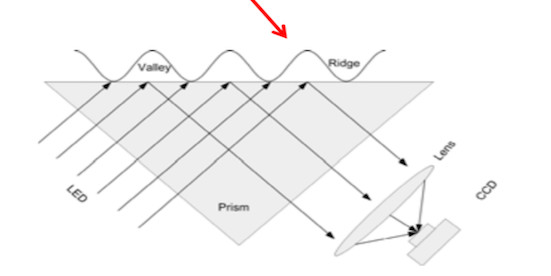
\includegraphics[scale=0.5]{fingerprintinflect.jpg}
	\caption{基于光学全反射原理的指纹在线采集技术。其原理就是当平行光通过三棱镜照在指纹上时,如果是凸起就不会发生反射,而如果是空气就会全反射。}
	\label{fig1}
	\end{figure}
	但是不管什么样采集方式,最后得到的图像大概就是下面这三种。\par 
	\begin{figure}[h!]
	\centering
	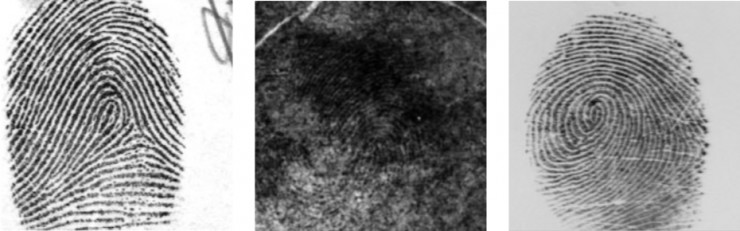
\includegraphics[scale=0.5]{picoffinger.jpg}
	\caption{从左到右分别为油墨指纹、来自现场的潜指纹和基于光学全反射原理的指纹}
	\label{fig2}
	\end{figure}
	指纹的质量决定了识别的准确率(当然其他生物特征的图像质量也是如此)。有很多原因会造成图像质量差。从传感器的角度来说,不同种类的传感器在分辨率、信噪比、面积大小等方面差异往往是很大的,这对采集到的信息的多少有很大影响。此外不同人的手指的皮肤状况也不一样,有的人皮肤太干燥或太潮湿,或者因为长期体力工作划痕比较多乳突纹被磨平,这都会造成采集质量较差。另外,当按手指时,按的方式和手的姿态也会对图像质量有影响。这些低质量指纹对于指纹识别算法都是很大的挑战。\par
	\noindent\textbf{二、图像的预处理和特征提取\citep{TinghuaUniversity}}\par 
	指纹的特征有比较清晰的定义,早些年没有自动指纹识别算法时指纹鉴定专家就利用这样的特征来做识别。这些特征依据分辨率大致可以分为三个层次。\par 

	\begin{itemize}
		\item 第一层:脊线方向和频率。即指纹的方向场和脊线的密集程度。脊线方向场中的奇异点也属于第一层特征,比如这个指纹的中央有两个奇异点。
		\item 第二层:脊线。当分辨率提高时,我们可以观察到脊线以及上面的一些特殊点(端点和分叉点),这也叫做细节点。
		\item第三层:脊线的内外轮廓。当分辨率再高一些可以观察到脊线并不是线,我们可以看到它有自己的外轮廓,中间还有一些白色空洞(即汗孔);不同手指上这些汗孔的位置和形态也存在差异。
	\end{itemize}

	现在的指纹识别系统主要利用的是前两层特征,因为第三层特征对于采集仪和手指皮肤的状况要求比较高,太过敏感。所以下面只介绍第一层和第二层特征的提取。通常的做法是先提取第一层特征,然后在第一层特征的指引下提取第二层特征。\par 
	\begin{figure}[h!]
	\centering
	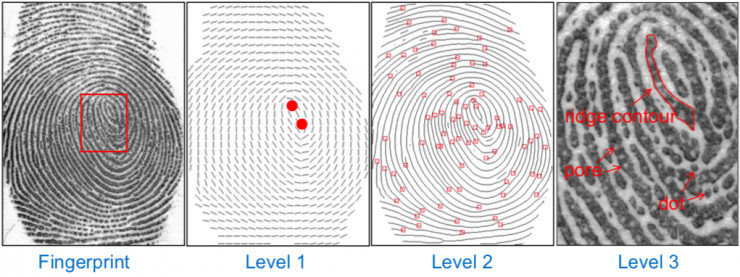
\includegraphics[scale=0.5]{cent.jpg}
	\caption{依据分辨率,指纹特征可以分为三层。}
	\label{fig3}
	\end{figure}
	~\\
	第一层特征提取\par
	\begin{figure}[h!]
	\centering
	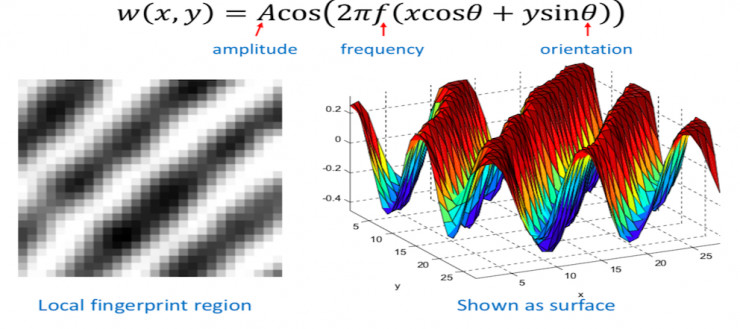
\includegraphics[width=4in]{cosdoble.jpg}
	\caption{将局部指纹图像显示为曲面}
	\label{fig4}
	\end{figure}
	在提取指纹的方向场和频率的时候,一般会做这样的假设,即指纹的局部图像可以用一个近似二维的正弦波来表示。通过这种局域分析方式分析每个小模块有一个问题,即在有噪声的地方会出错。解决的方法就是做方向场的平滑。具体就如上图所示,先将向量场分解成向量的正弦和余弦,然后分别对这两个图像做平滑,最后再将平滑过的两个图像还原成平滑的方向场。\par ~\\
	第二层特征提取  ~\\ \par 
		有了方向场和频率之后,接下来就是做脊线的提取。但是由于脊线上有相对比较明亮的汗孔,或者由于干裂等导致的脊线断裂,或者由于手指潮湿使得相邻脊线粘连等原因,脊线一般不能够进行直接提取,而需要先做增强。\par


	针对一般图像的增强方法对于指纹来说效果通常不是很好;在指纹增强中比较有效的方法是「上下文滤波」,一个典型的方法就是Gabor滤波器。Gabor滤波器本身是一个复滤波器,指纹增强只用到它的实部。从上图可以看出,经过Gabor滤波之后,指纹图像上的脊线不再有汗孔,粘连的脊线也会分开,断裂的地方也会连起来。由于指纹各处脊线的方向和频率不同,每个位置到底该用哪种参数的Gabor滤波器,是需要按照该位置的方向以及频率来挑选的。\par


	然后就可以对这些增强图用传统的阈值化方法得到二值图像,再对它做形态学处理,可以得到细化图;通过分析细化图可以检测出来上面的端点以及分叉点,还可以进一步推断出来这些细节点的方向。\par 

	最后,指纹图像的质量通常不是理想的,所以即便经过前面的增强,做了细化和细节点提取,但总还会出现一些假的细节点,所以还需要做一步细节点的验证,这一步会识别出很多典型的伪细节点,比如图像边缘的伪细节点、成对出现的方向相反的伪细节点等。通过这些规律可以尽量把伪细节点去掉。\par 

	\noindent\textbf{三、匹配}\par 

	大部分指纹匹配算法是基于细节点的匹配,所以这个步骤就是一个点匹配的问题。\par 
	\begin{figure}[h!]
	\centering
	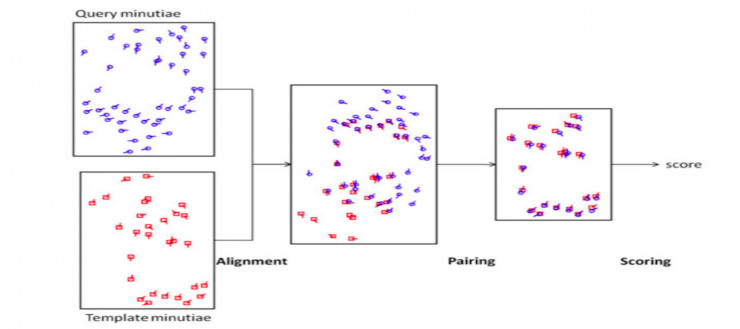
\includegraphics[scale=0.5]{KMP.jpg}
	\caption{细节点匹配}
	\label{fig5}
	\end{figure}
	跟一般的点匹配不同的是,指纹细节点是带方向的;细节点的类型(端点或者分叉点)用的比较少,因为点的类型不是特别稳定。\par 

	做细节点匹配的时候,很重要的一个步骤就是指纹的对齐。指纹识别与人脸识别或虹膜识别不太一样,它的姿态不好确定,所以拿到两个图像之后只能找到一个相对的旋转和平移关系,只是相对对齐,而人脸和虹膜可以做绝对的对齐。指纹对齐之后就可以找到对应点,然后通常某种方法算出匹配分数。\par 



\section{进一步的思考}
% 结合学习的计算科学知识,对分组演讲涉及的问题作进一步的思考。\par
	生物识别作为一项我们在日常生活中必不可少的技术,他的未来前景是怎样的呢?\par 
	出于对安全性的考虑,对于目前大多数在云端的识别,更主张在设备执行更多操作(也就是边缘处理)即只有不像原始生物数据那样的敏感信息才会上传,这样对云端来说降低了负荷,对整体用户来说降低了数据泄密的风险,对入侵者来说提高了他们非法获取信息的成本。同时,基于边缘处理的生物识别对个人用户设备的安全性提出了更高的要求。\par 
	通过对冯建江教授的《指纹识别现状与研究进展》报告及其他资料,结合老师给出的最近大热的人工智能领域,发现Deep Learing(深度学习)与指纹识别技术结合可以极大的降低成本,实现节俭学习即通过较少的数据学习得到更优的效果可以有效地节约人力物力财力,那么关于人工智能它是如何和指纹识别建立联系呢?\par 
	要想进行指纹识别首先面临的难题就是如何区分背景和指纹,当在受控环境中(如使用轻型或电容式扫描仪)进行采集时,背景更容易检测,因为可以进行多次扫描试验,直到获得满意的结果。由于印刷污染,潜伏印刷中的情况(那些留在场景中)更难处理。打印污染可能是由于灰尘、油、血、粗糙表面和其他液体的采集造成的,这些液体遮蔽了打印,因此很难将背景与打印中包含的信息区分开来。因此,指纹分割是指纹采集和识别的关键第一步。自动指纹识别分割算法应用局部均值和方差标准来分解图像,可以使用机器学习方法。根据打印的前景和背景区域中的局部均值和方差分布,对分类器进行训练。神经网络对于这一二进制分类问题尤为成功,因为不需要复杂的网络架构,在平均方差空间中,只有很少的感知器能够实现背景和前景的合理区分\citep{devidefingerpeint}。\par 

	随着越来越多的智能设备走进人们的生活,智能手机等小型化设备普遍面临着一个共同的问题小面积指纹识别的准确率明显下降\citep{littefingerprint}。过去指纹识别的特征点及图像主要由人来规定,现在可以有人工智能进行分类器的选取,基于这个思路,可以对过去的指纹识别系统进行升级,通过构建卷积神经网络来进行分类器的筛选,进而实现节俭学习。\par 

	对于生物识别从哲学方面来说,只要存在生物信息的交换就存在泄露的风险,那么我们可以采用较少的敏感数据获得较高的安全级别。数字行为的生物识别提供了很好的解决方案,用键盘输入方式、数字签名等来对个人匹配。同时,短期的生物特征,比如穿衣、配饰、发色等也可用于识别认证。\par 
	对于整体行业行业,虹膜识别正在蓬勃发展大有取代指纹识别和人脸识别的地位的趋势,这是基于他原理和识别精度较人脸识别和指纹识别有较大的优势(普遍地来说,指纹识别的识别率错误率在0.8\%人脸识别2\%虹膜识别仅有千万分之一)\par

% 这里是简单列表的样例:(如果需要标号自定义或者自动标记数字序号,请自行搜索语法)
% \begin{itemize}
%     \item 简单的列表结构 
%     \item 如这里所示
%     \item 此处仅为样例
%     \item 按需修改和使用
% \end{itemize}


\section{总结}
	对于现在来社会来说,信息化、虚拟化是一个必然的趋势,个人与互联网的联系必将越来越密切。从另一方面来说,我们的个人信息、资料面临着泄露的潜在风险。那么如何保障我们的个人隐私安全呢?我认为生物识别可能会是一条出路,同时这条路也面临着重重挑战。随着越来越多的技术人员将目光投向生物识别,过去的模式识别模式是否依旧安全?我们的个人生物信息是否可能被窃取利用?都是值得深思的问题。这条路必然充斥着攻防的相互对垒,当我相信它的前景是光明的。每一次成功的骇入都促进了新的安全技术的产生。\par 
	通过计算机科学导论的学习,我明白了不能人云亦云,看破了人工智能神秘的面纱,通俗的来讲,就目前而言人工智能并没有是我们想象的那么智能,本质上他只不过是通过不断地训练对可能发生的事件通过统计学及微积分知识进行最大可能性的选择。而有些别有用心的人利用这些新的名词来唬人吸金赚取财富,最后跑跑坑害了消费者和投资人的财力和感情,只会让计算机这个学科蒙上阴霾,自设囚笼,最终只会坑害自己。\par 
	同时老师的不断教诲也让我明白了这样一个道理:我们是祖国的新一代,我们的生活不是上天赐予的,而是成千上万的中国人他们用自己的知识、血肉为我们夺取的和平生活,当今世界美国的霸权主义盛行,依旧主张用绝对的武力巩固自己的统治。中国正在崛起,毫无疑问触及到了他强盛的生命线,在这种情况下,中美关系势必紧张。而之前的5G之争鲜明的论证了这一观点。我们若想挺胸抬头做人,做中国人,必须发展高精尖技术进而打破美国的科技封锁,为此身为祖国的热血青年的一份子,我们加强对前沿技术和国际形势的了解具有重要意义。而这门课程恰恰提供了机会,让我们了解前沿科技做命运的掌舵人。\par 


\section{附录}
\begin{itemize}
    \item Github https://github.com/KVM-Explorer
    	\begin{figure}[H]
		\centering
		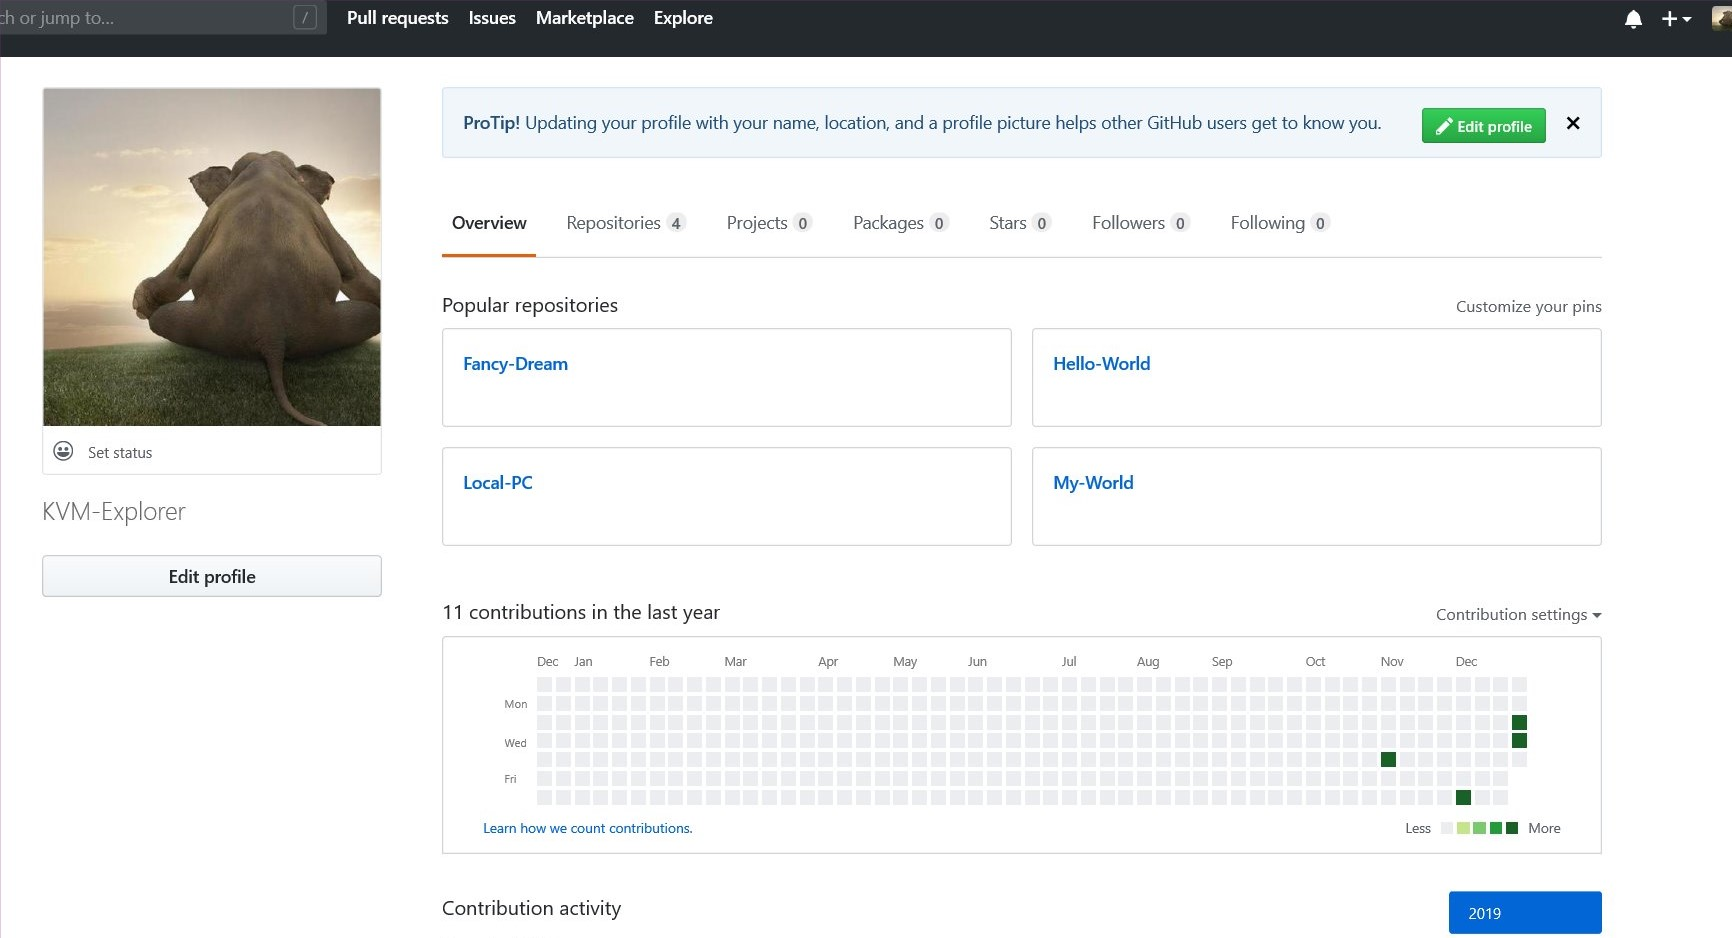
\includegraphics[width=5in,height=3in]{github.jpg}
		\caption{Github}
		\end{figure}
    \item 观察者
    	\begin{figure}[H]
		\centering
		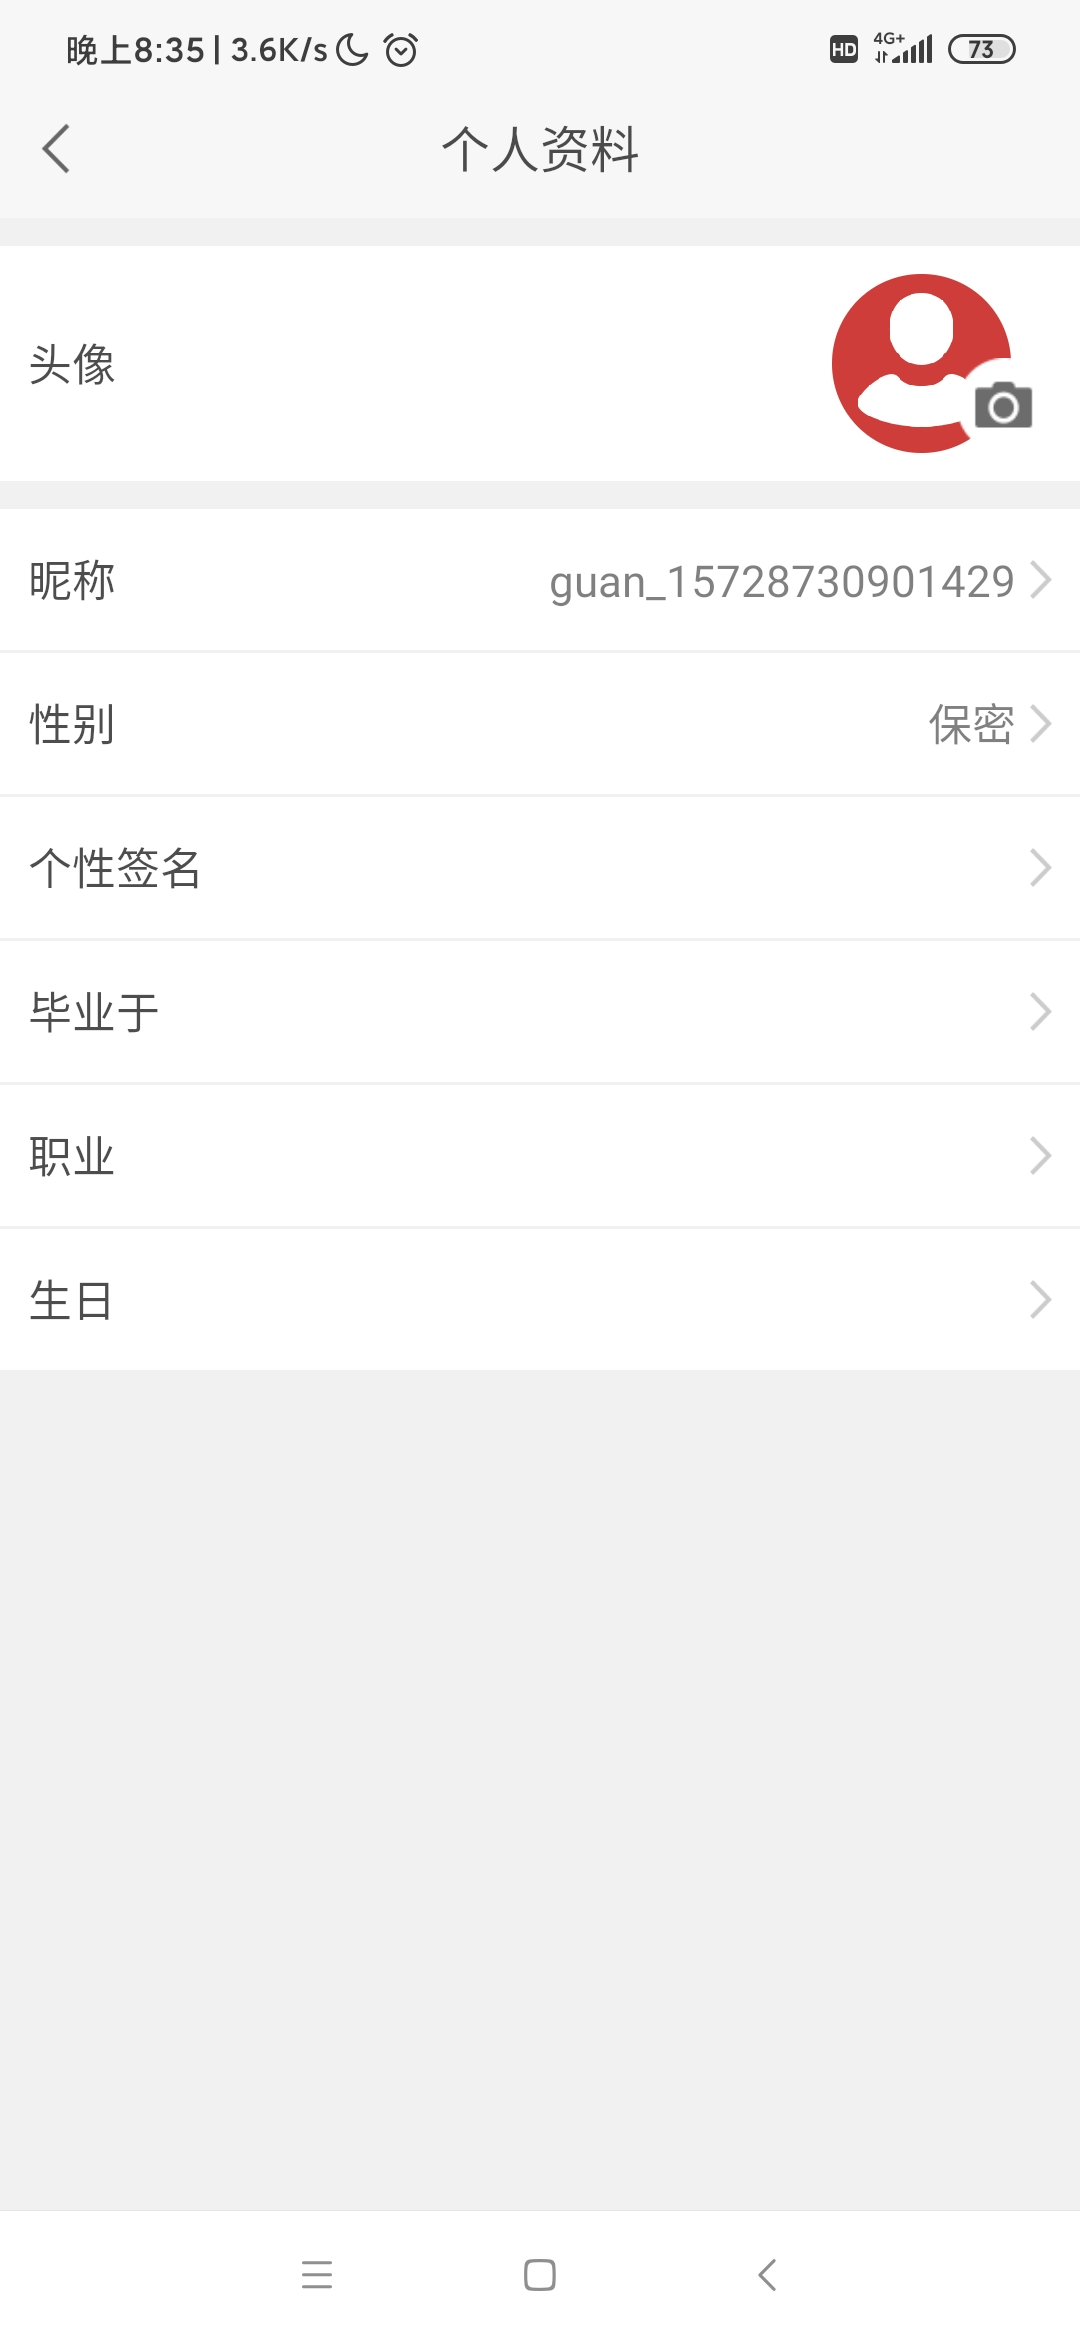
\includegraphics[height=4in,width=3in]{guanchazhe.jpg}
		\caption{观察者}
		\label{fig2}
		\end{figure}
	\item 学习强国
		\begin{figure}[H]
		\centering
		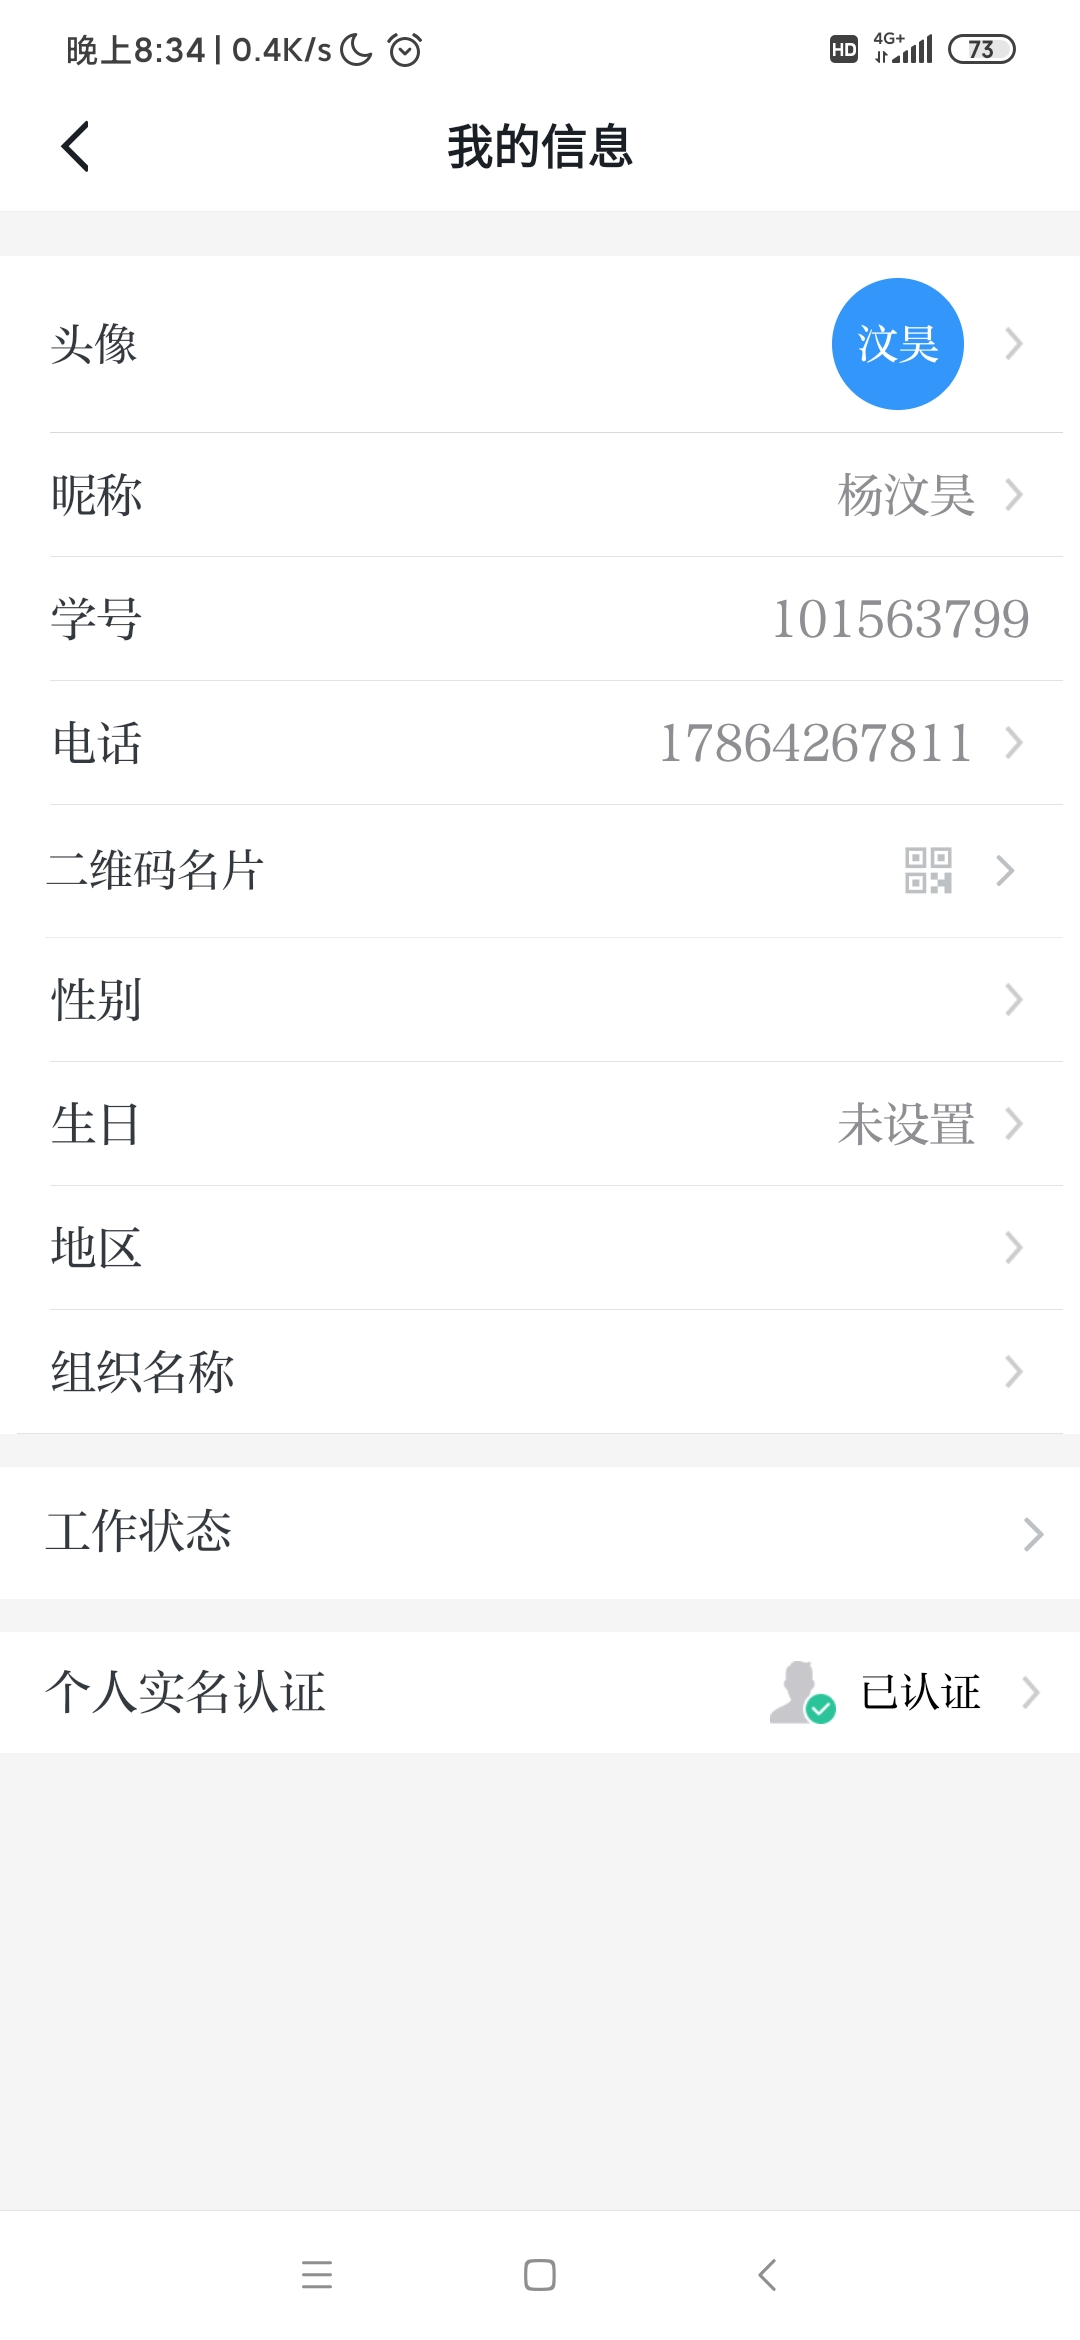
\includegraphics[height=3in,width=3in]{xuexiqiangguo.jpg}
		\caption{学习强国}
		\label{fig3}
		\end{figure}
	\item 哔哩哔哩
		\begin{figure}[H]
		\centering
		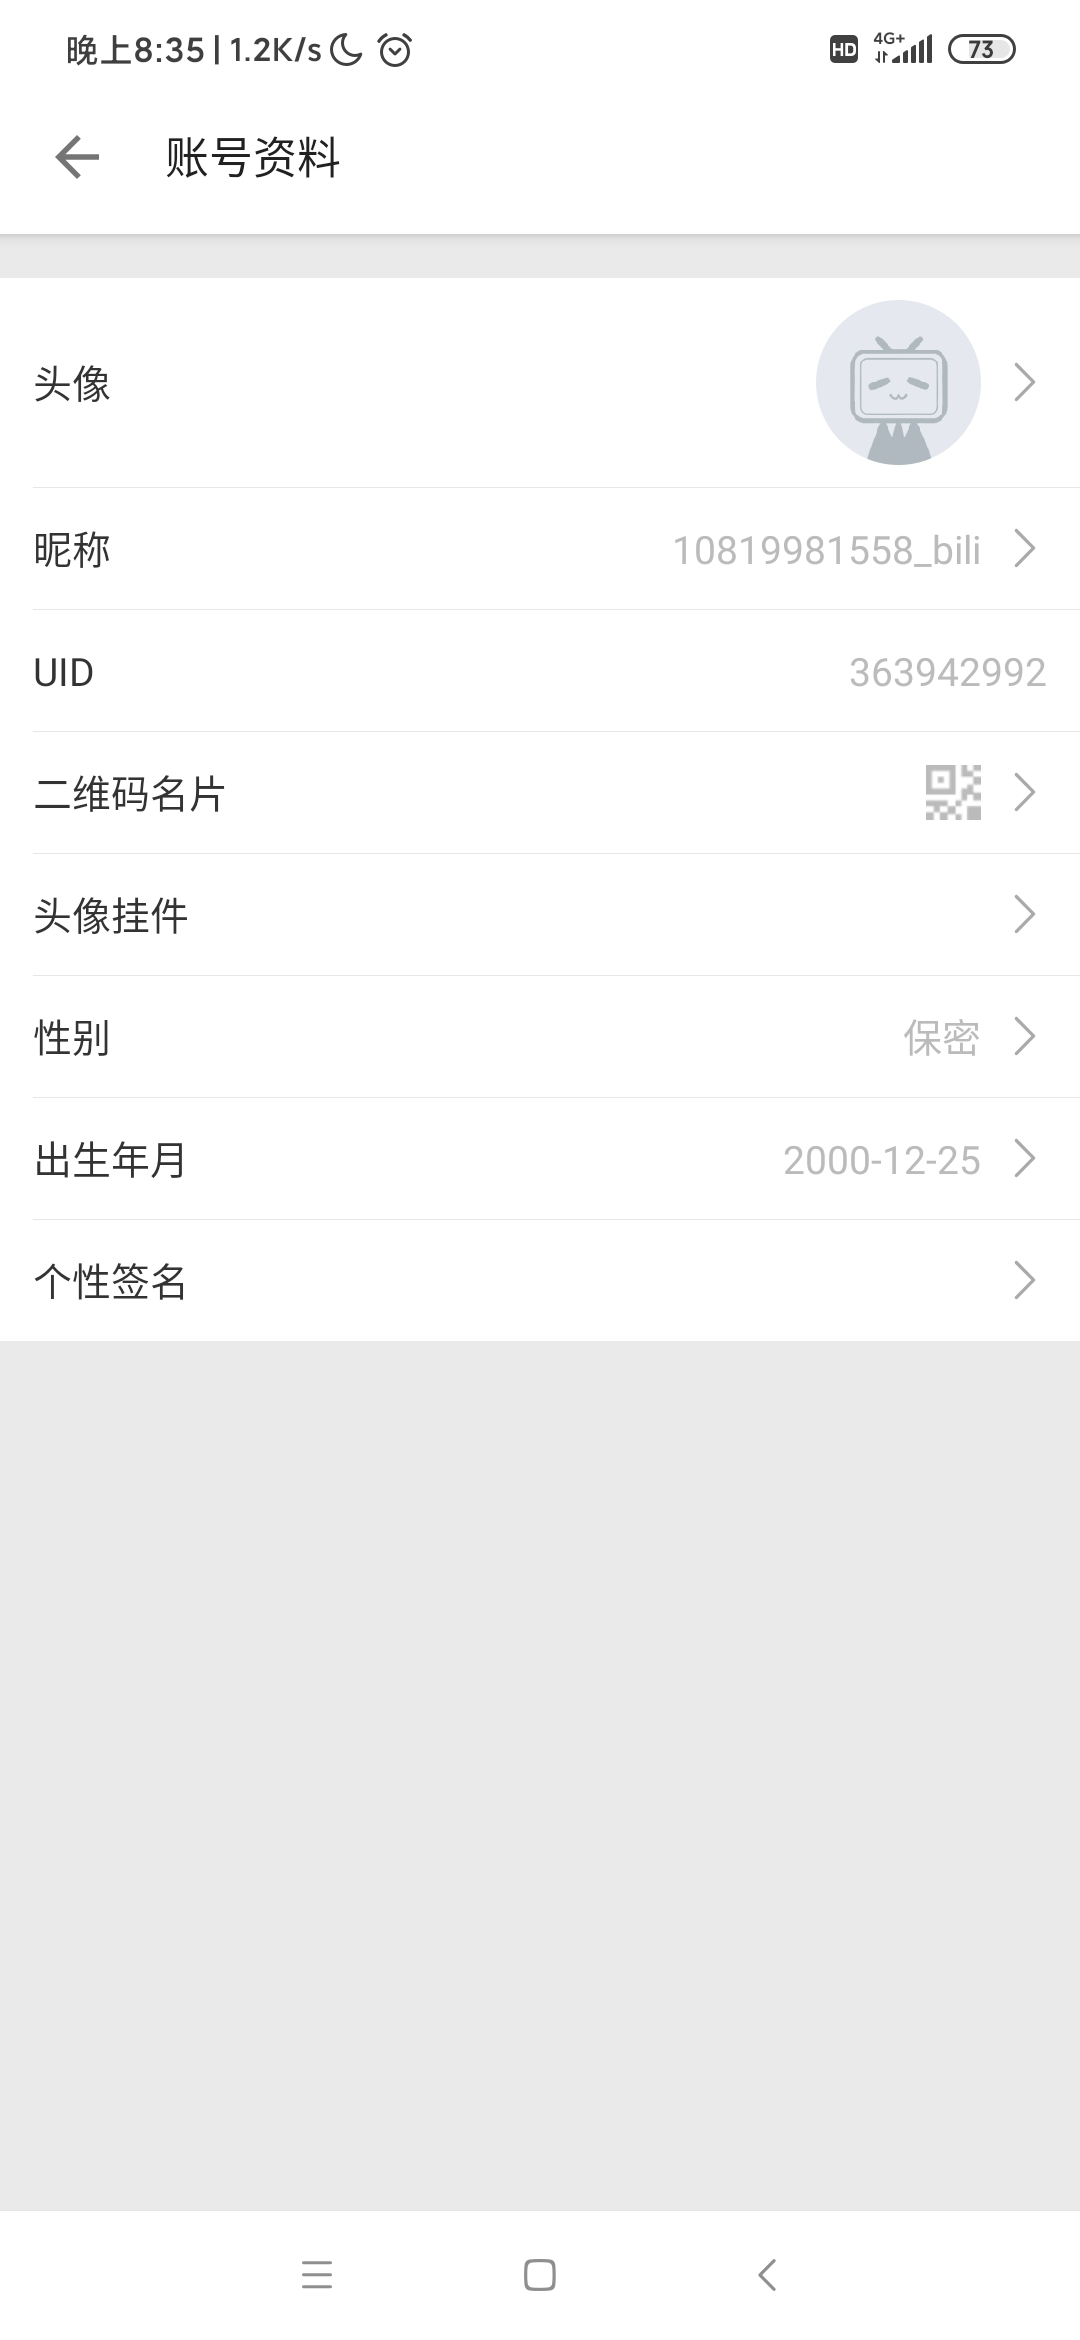
\includegraphics[height=3in,width=3in ]{Bzhan.jpg}
		\caption{哔哩哔哩}
		\label{fig4}
		\end{figure}
    \item 博客园 http://home.cnblogs.com/u/KVMX/
    	\begin{figure}[H]
		\centering
		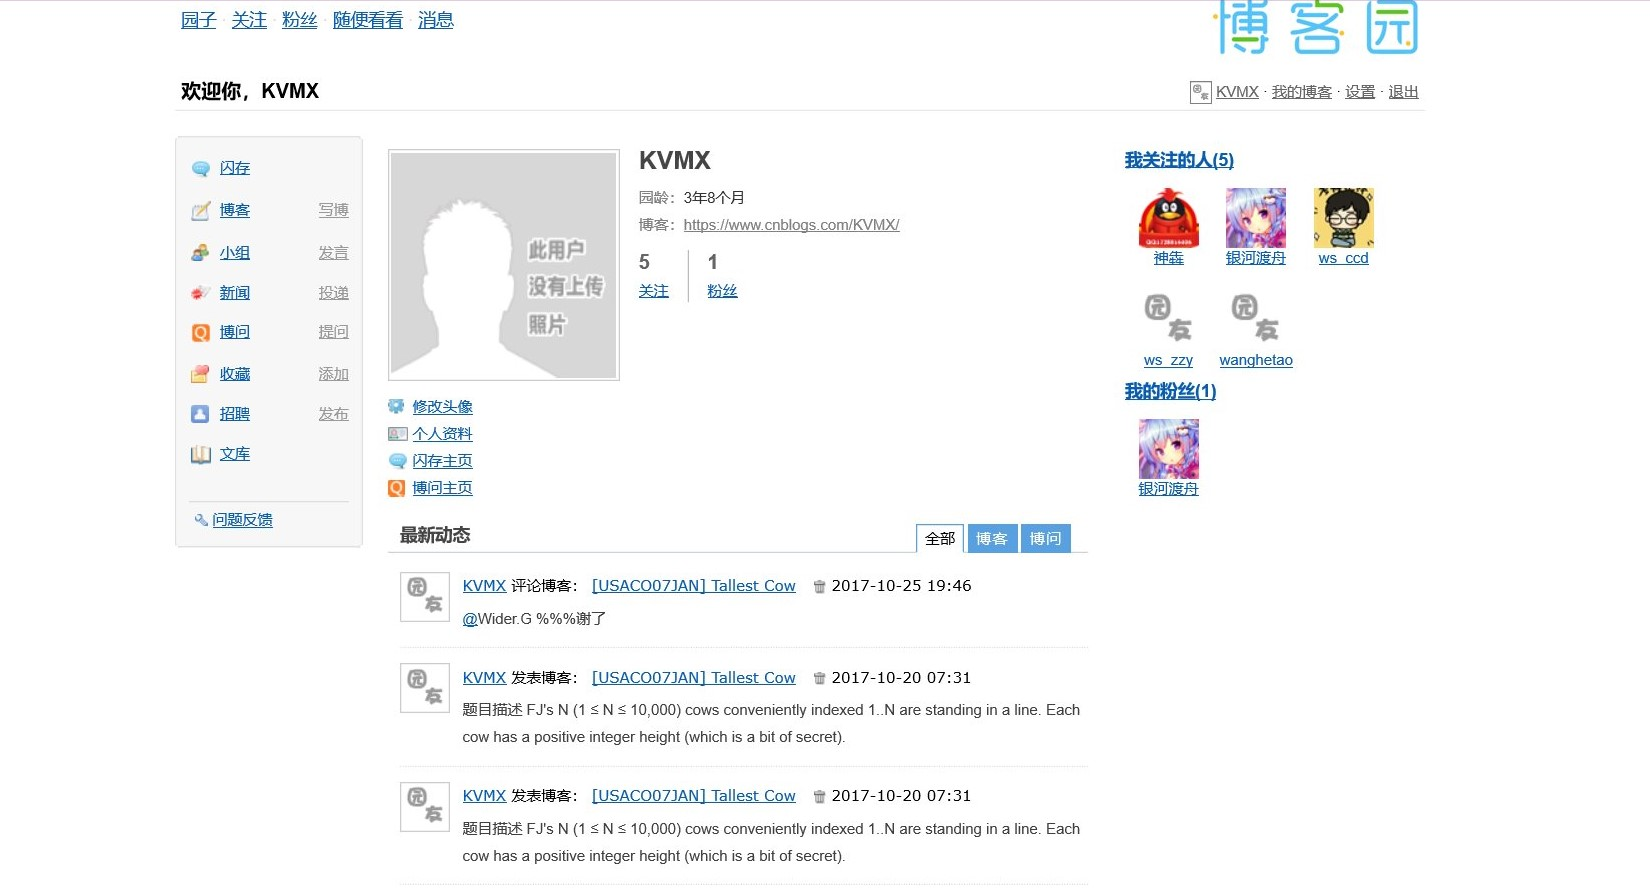
\includegraphics[width=5in]{bokeyuan.jpg}
		\caption{博客园}
		\label{fig5}
		\end{figure}
    \item CSDN https://i.csdn.net/\#/uc/profile
    	\begin{figure}[H]
		\centering
		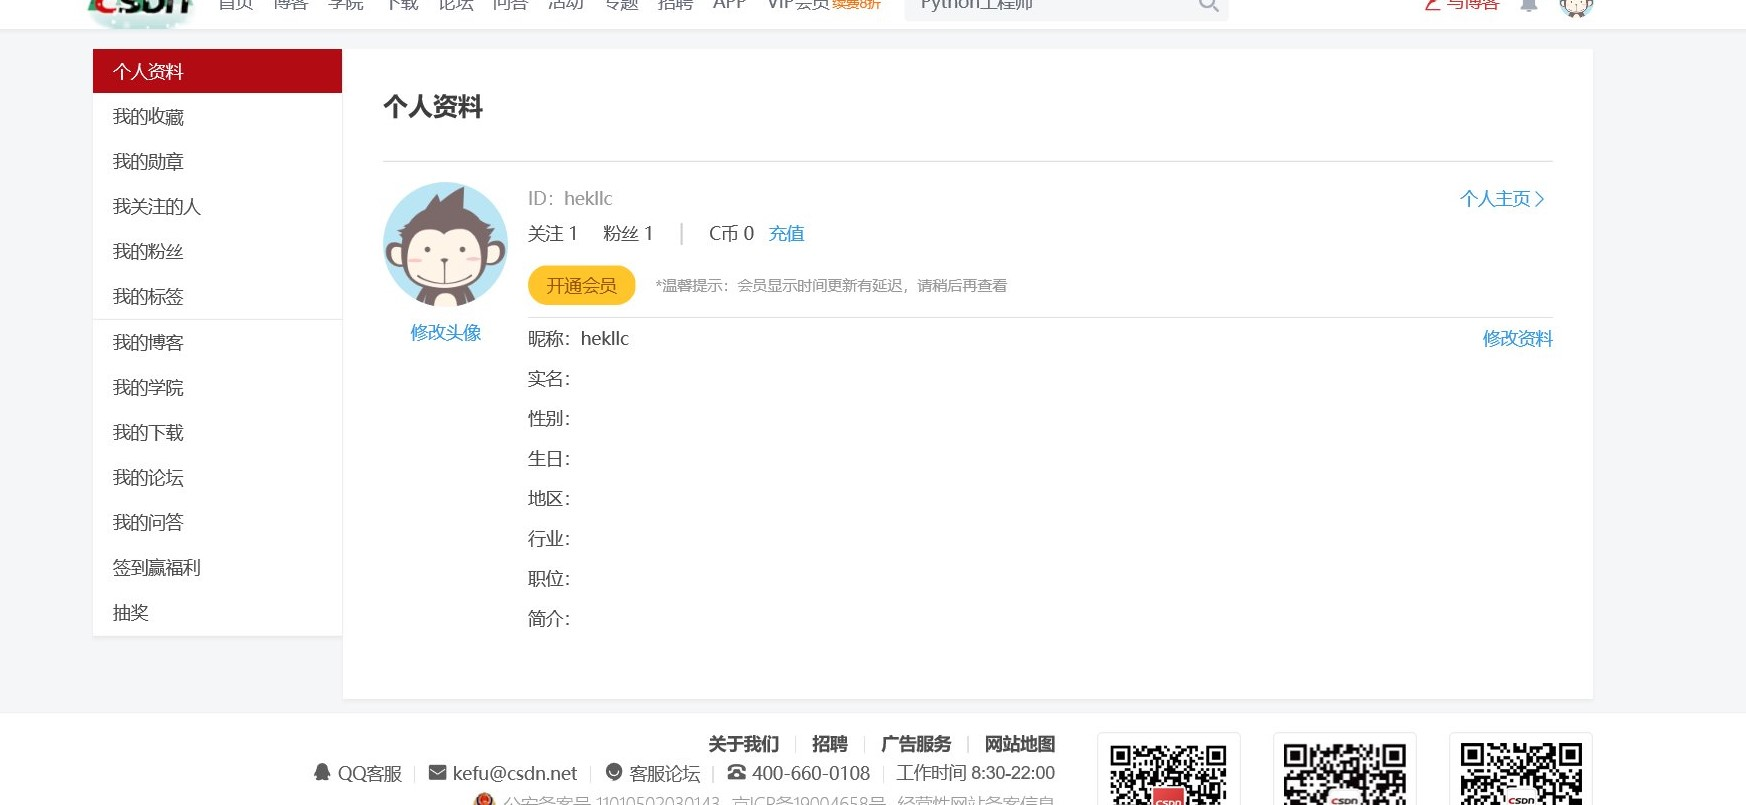
\includegraphics[width=5in]{CDSDN.jpg}
		\caption{CSDN}
		\label{fig6}
		\end{figure}
    \item 小木虫 http://muchong.com/bbs/space.php?uid=20262666
    	\begin{figure}[H]
		\centering
		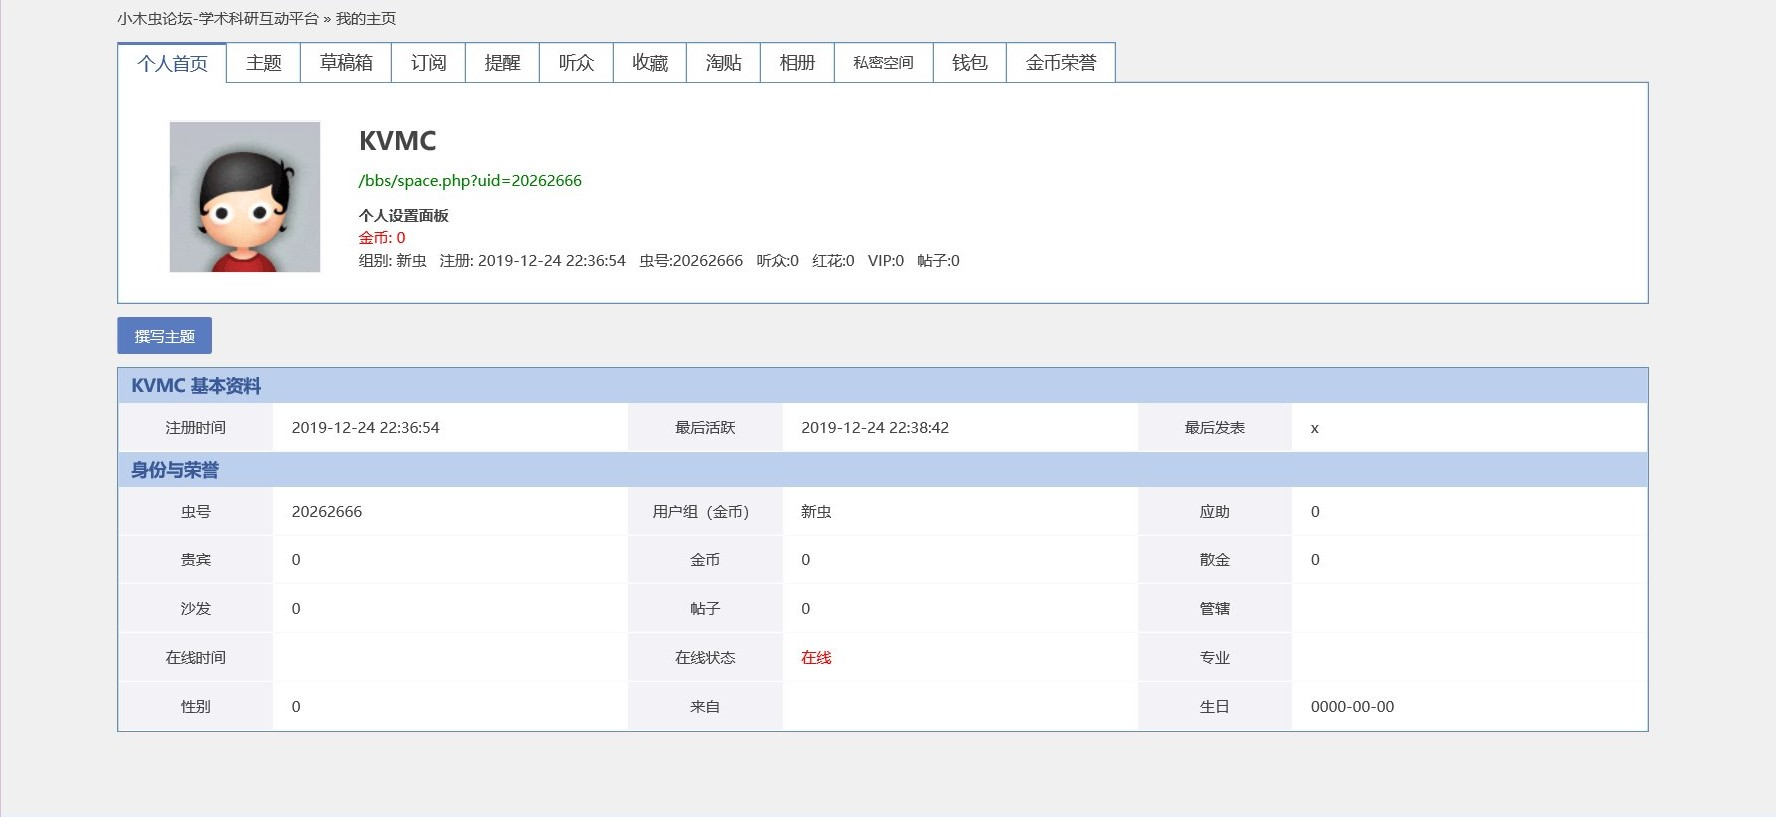
\includegraphics[width=5in]{littlepeat.jpg}
		\caption{小木虫}
		\label{fig7}
		\end{figure}

\end{itemize}


\hspace*{\fill} \\

% {\bf 注意,参考文献至少五篇,其中至少两篇为英文文献,参考文献必须在正文中有引用。}
\bibliographystyle{plain}
\bibliography{references}


\end{document}
